\documentclass[12pt,a4paper]{article}
\usepackage{geometry}
\usepackage[numbers]{natbib}
\usepackage{amssymb, amsmath}
\usepackage{graphicx}
\usepackage{grffile}
\graphicspath{{../Figures/}}
\usepackage{gensymb}
\usepackage[font=small]{caption}
\usepackage[utf8]{inputenc}
\usepackage[english]{babel}
\usepackage{fancyhdr}
\usepackage[raggedright]{titlesec}
\usepackage{subcaption}
\usepackage{multirow}
\usepackage{dirtytalk}
\usepackage{framed}
\usepackage[pdftex,breaklinks]{hyperref}
\hypersetup{
  colorlinks   = true, %Colours links instead of ugly boxes
  urlcolor     = green, %Colour for external hyperlinks
  linkcolor    = blue, %Colour of internal links
  citecolor   = red %Colour of citations
}


\begin{document}
\author{Katrina Ashton}


\pagestyle{fancy}
\fancyhf{}
\rhead{\thepage}
\lhead{u5586882}

\section{What I've done}
\begin{itemize}
\item{Looked at the point cloud registration one frame at a time}
\item{Started reading those papers you sent me and some ICP surveys}
\item{Installed PCL (1.8, Windows). Although I haven't used it yet so not 100\% sure it'll work.}
%\item{Added more to the appendices for the final report draft}
\end{itemize}

\section{Parts of report to look at}
\begin{itemize}
\item{Nothing new.}
\end{itemize}

\section{Questions}
\begin{itemize}
\item
\end{itemize}

\section{Comments}
\begin{itemize}
\item One of the ICP surveys linked to their open-source library: \url{https://github.com/ethz-asl/libpointmatcher}. This has modular implementations for various methods to do each of the steps of ICP. Might be a good place to start looking. Compilation on windows isn't fully supported so I might have to switch over to ubuntu while coding if I end up using it.
\item I realised that the registered point cloud I've included in my previous report is actually only two point clouds. The full one is much worse, and has two distinct clusters that are very far apart, and are each made up of a few closer clusters (see figure \ref{f: all registered}). The registration between each point cloud also seems pretty poor.
\end{itemize}

\begin{figure}[b!]
  \centering
  \begin{subfigure}[t]{0.5\textwidth}
  \centering
    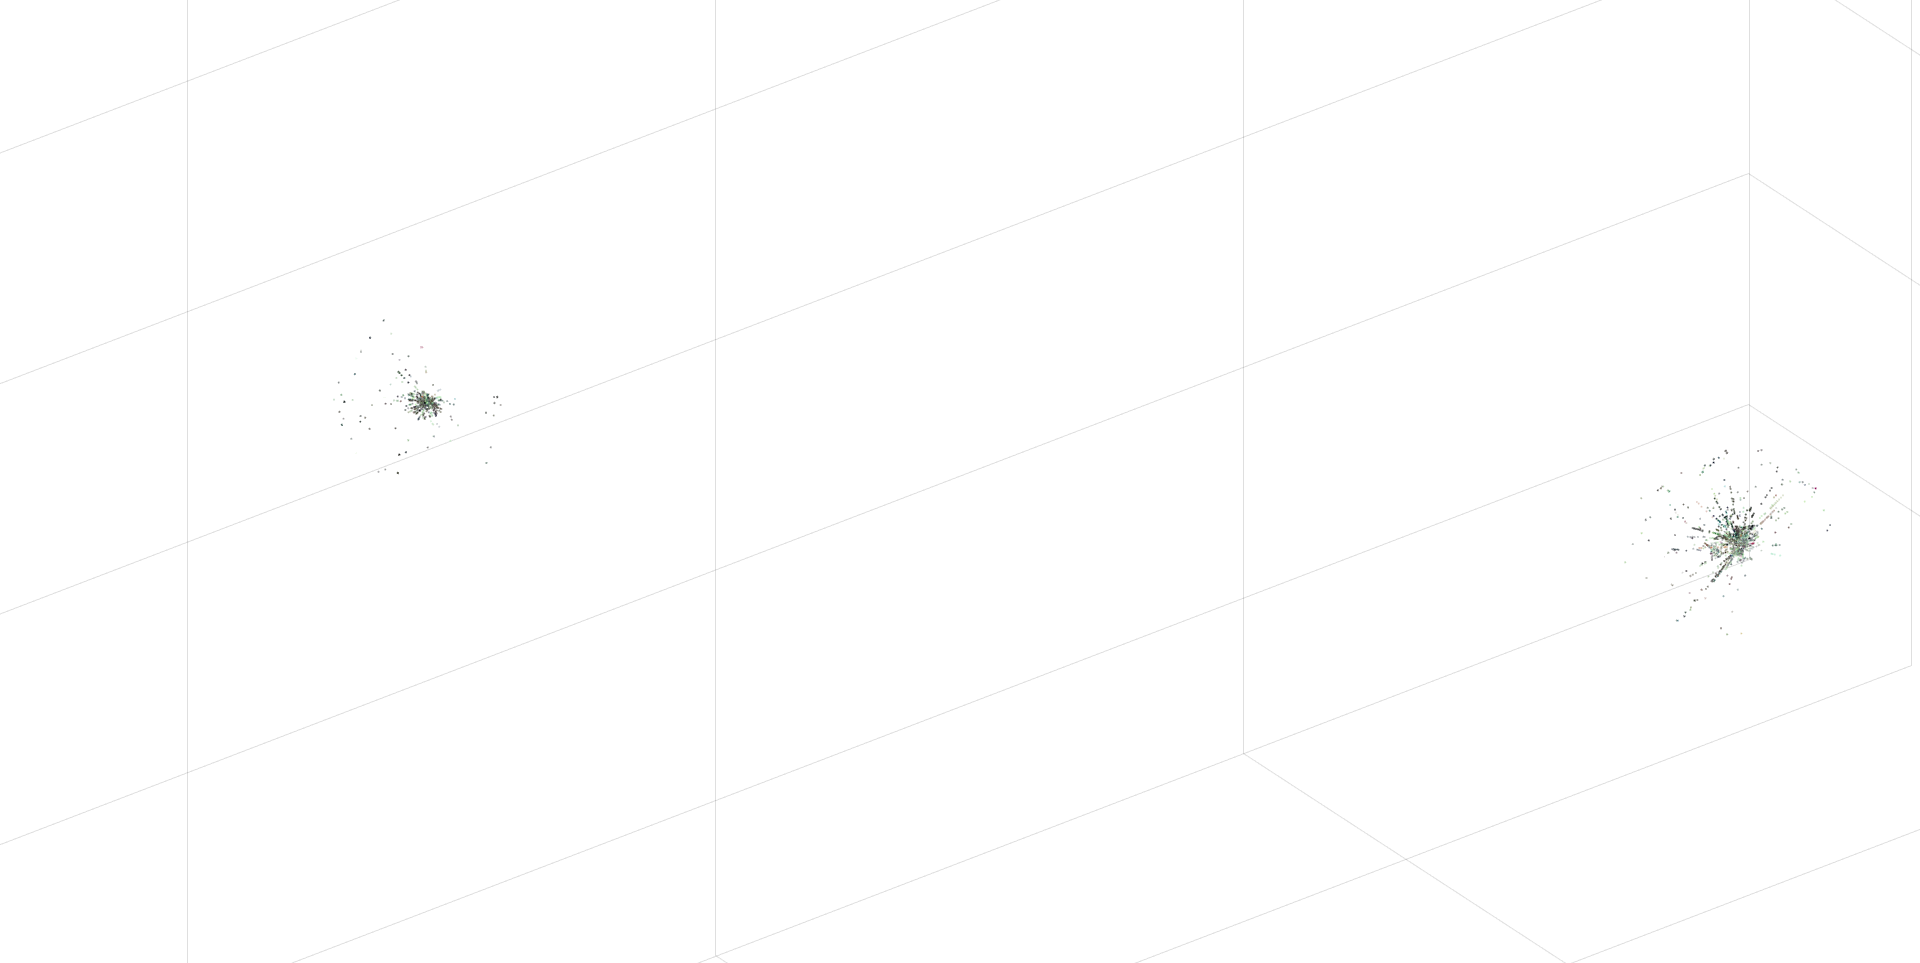
\includegraphics[width=60mm, trim =0mm 0mm 0mm 0mm, clip]{two_clusters.png}
  \caption{All points of registered point cloud. Note two distinct clusters.}
  \end{subfigure}
  \\
  \begin{subfigure}[t]{0.5\textwidth}
  \centering
    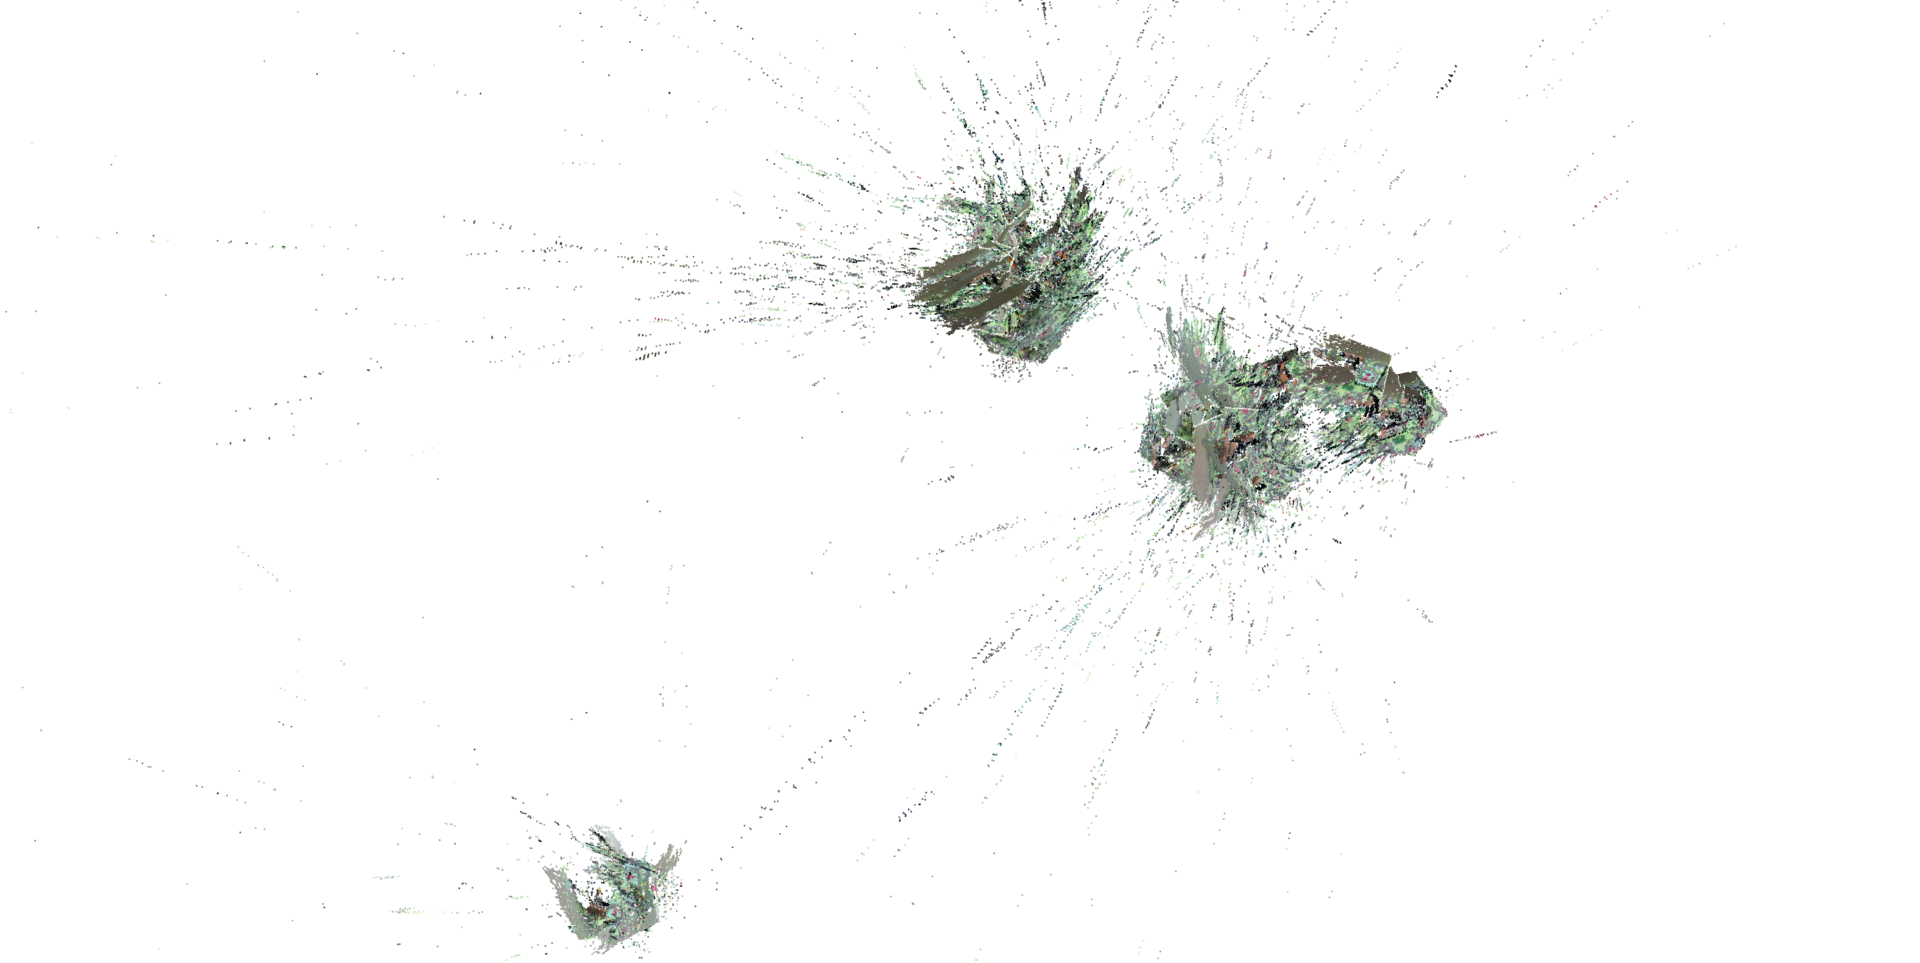
\includegraphics[width=60mm, trim =0mm 0mm 0mm 0mm, clip]{cluster1.png}
  \caption{Zoom-in on right cluster}
  \end{subfigure}%
  ~
  \begin{subfigure}[t]{0.5\textwidth}
  \centering
    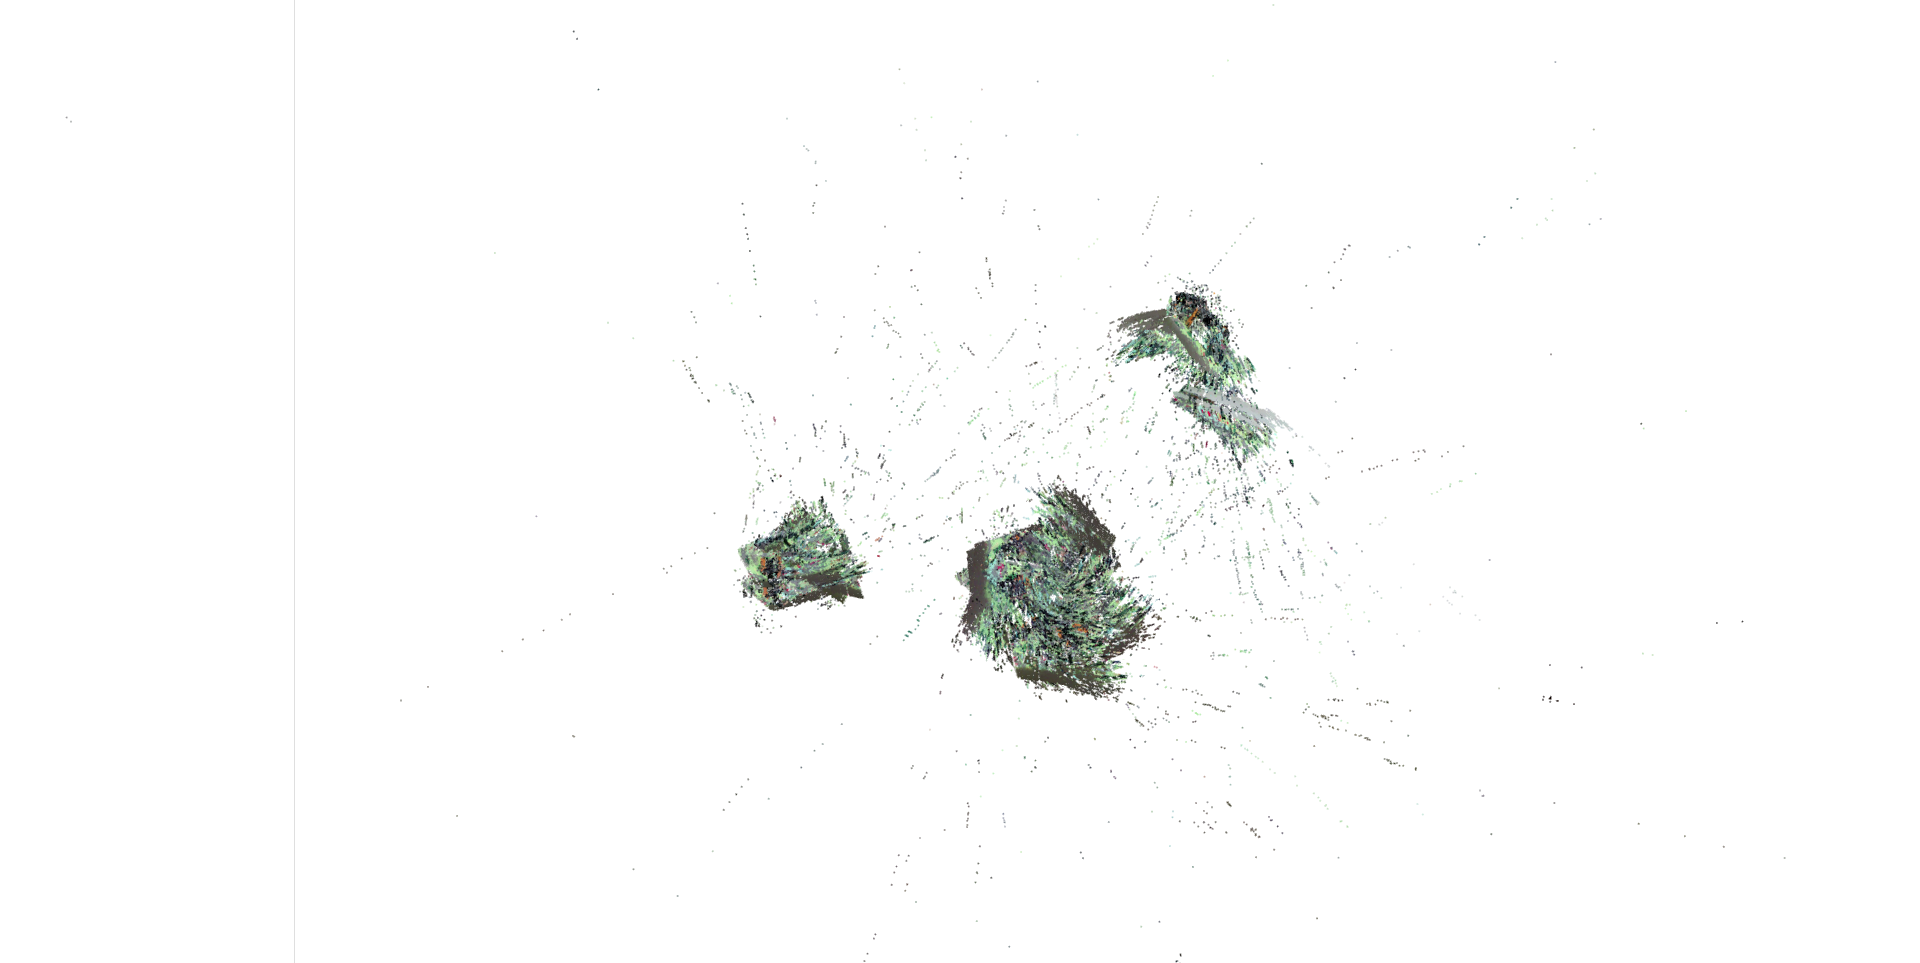
\includegraphics[width=60mm, trim =0mm 0mm 0mm 0mm, clip]{cluster2.png}
  \caption{Zoom-in on left cluster}
  \end{subfigure}
  \caption{All point clouds registered using MATLAB.}
  \label{f: all registered}
\end{figure}

\end{document}